% Options for packages loaded elsewhere
\PassOptionsToPackage{unicode}{hyperref}
\PassOptionsToPackage{hyphens}{url}
%
\documentclass[
  ignorenonframetext,
]{beamer}
\usepackage{pgfpages}
\setbeamertemplate{caption}[numbered]
\setbeamertemplate{caption label separator}{: }
\setbeamercolor{caption name}{fg=normal text.fg}
\beamertemplatenavigationsymbolsempty
% Prevent slide breaks in the middle of a paragraph
\widowpenalties 1 10000
\raggedbottom
\setbeamertemplate{part page}{
  \centering
  \begin{beamercolorbox}[sep=16pt,center]{part title}
    \usebeamerfont{part title}\insertpart\par
  \end{beamercolorbox}
}
\setbeamertemplate{section page}{
  \centering
  \begin{beamercolorbox}[sep=12pt,center]{part title}
    \usebeamerfont{section title}\insertsection\par
  \end{beamercolorbox}
}
\setbeamertemplate{subsection page}{
  \centering
  \begin{beamercolorbox}[sep=8pt,center]{part title}
    \usebeamerfont{subsection title}\insertsubsection\par
  \end{beamercolorbox}
}
\AtBeginPart{
  \frame{\partpage}
}
\AtBeginSection{
  \ifbibliography
  \else
    \frame{\sectionpage}
  \fi
}
\AtBeginSubsection{
  \frame{\subsectionpage}
}
\usepackage{amsmath,amssymb}
\usepackage{lmodern}
\usepackage{ifxetex,ifluatex}
\ifnum 0\ifxetex 1\fi\ifluatex 1\fi=0 % if pdftex
  \usepackage[T1]{fontenc}
  \usepackage[utf8]{inputenc}
  \usepackage{textcomp} % provide euro and other symbols
\else % if luatex or xetex
  \usepackage{unicode-math}
  \defaultfontfeatures{Scale=MatchLowercase}
  \defaultfontfeatures[\rmfamily]{Ligatures=TeX,Scale=1}
\fi
% Use upquote if available, for straight quotes in verbatim environments
\IfFileExists{upquote.sty}{\usepackage{upquote}}{}
\IfFileExists{microtype.sty}{% use microtype if available
  \usepackage[]{microtype}
  \UseMicrotypeSet[protrusion]{basicmath} % disable protrusion for tt fonts
}{}
\makeatletter
\@ifundefined{KOMAClassName}{% if non-KOMA class
  \IfFileExists{parskip.sty}{%
    \usepackage{parskip}
  }{% else
    \setlength{\parindent}{0pt}
    \setlength{\parskip}{6pt plus 2pt minus 1pt}}
}{% if KOMA class
  \KOMAoptions{parskip=half}}
\makeatother
\usepackage{xcolor}
\IfFileExists{xurl.sty}{\usepackage{xurl}}{} % add URL line breaks if available
\IfFileExists{bookmark.sty}{\usepackage{bookmark}}{\usepackage{hyperref}}
\hypersetup{
  pdftitle={Comparing cross-language phonological profiles},
  hidelinks,
  pdfcreator={LaTeX via pandoc}}
\urlstyle{same} % disable monospaced font for URLs
\newif\ifbibliography
\usepackage{graphicx}
\makeatletter
\def\maxwidth{\ifdim\Gin@nat@width>\linewidth\linewidth\else\Gin@nat@width\fi}
\def\maxheight{\ifdim\Gin@nat@height>\textheight\textheight\else\Gin@nat@height\fi}
\makeatother
% Scale images if necessary, so that they will not overflow the page
% margins by default, and it is still possible to overwrite the defaults
% using explicit options in \includegraphics[width, height, ...]{}
\setkeys{Gin}{width=\maxwidth,height=\maxheight,keepaspectratio}
% Set default figure placement to htbp
\makeatletter
\def\fps@figure{htbp}
\makeatother
\setlength{\emergencystretch}{3em} % prevent overfull lines
\providecommand{\tightlist}{%
  \setlength{\itemsep}{0pt}\setlength{\parskip}{0pt}}
\setcounter{secnumdepth}{-\maxdimen} % remove section numbering
%\ProvidesPackage{config/presento}
\mode<presentation>

% removing navigation symbols
\setbeamertemplate{navigation symbols}{}

% packages
\usepackage{xcolor}
\usepackage{fontspec}
\usepackage{setspace}
\usepackage{tikz}
\usepackage{multicol}
\usepackage{multirow}
\usepackage{philex}

% colors
\definecolor{colorblack}{HTML}{000000} % for note
\definecolor{colorgreen}{HTML}{009933} % for code
\definecolor{colorwhite}{HTML}{FFFFFF} % background
\definecolor{colorblue}{HTML}{0099CC} % blue
\definecolor{colorbig}{HTML}{1f77b4} % for note
\definecolor{colormedium}{HTML}{ff7f0e} % for note
\definecolor{colorsmall}{HTML}{2ca02c} % for note


% font sizes
\newcommand{\fontsizeone}{1em}
\newcommand{\fontsizetwo}{1em}
\newcommand{\fontsizethree}{0.8em}
% line spaces
\newcommand{\linespaceone}{1}

% font families
\newfontfamily{\inconsolatafont}[Path=fonts/]{brill}

% beamer template changes
\setbeamertemplate{frametitle}{
 \vspace{0.40em}
 \noindent
 \hspace{-1.22em}
 \tikz[overlay,remember picture,baseline=0.3em]{\fill[fill= colorblue]  (-0.3,0.05) rectangle (0,0.9); }\color{colorblue}~~\insertframetitle%
}

\setmainfont[Ligatures=TeX,Path=fonts/,
						BoldFont=brillb,
						ItalicFont=brilli,
						BoldItalicFont=brillbi,
						SmallCapsFont=brill]{brill}
\setsansfont[Ligatures=TeX,Path=fonts/,
						BoldFont=brillb,
						ItalicFont=brilli,
						BoldItalicFont=brillbi,
						SmallCapsFont=brill]{brill}
\setmonofont[Scale=0.7,
  						   Path=fonts/]{iosevka-regular}
  
\usepackage[english,russian]{babel}
						
\newfontfamily\tgtermes{TeX Gyre Termes}

\makeatletter
  \begingroup
    \tgtermes
    \DeclareFontShape{\f@encoding}{\rmdefault}{m}{sc}{%
      <-> ssub * \f@family/m/sc}{}
    \DeclareFontShape{\f@encoding}{\rmdefault}{bx}{sc}{%
      <-> ssub * \f@family/bx/sc}{}
  \endgroup
\makeatother

% frame counter
\newcounter{totalfr}
\setbeamertemplate{footline}{
  \ifnum\inserttotalframenumber=1
    \setcounter{totalfr}{2}
  \else
     \setcounter{totalfr}{\inserttotalframenumber}
  \fi
  \hfill{
    \tikz{
      \filldraw[fill=colorblue!80, draw=colorblue!80]  (0,0) -- (0.2,0) arc (0:{\value{framenumber}*(360/(\value{totalfr}))}:0.2) -- (0,0); 
      \node at (0,0) {\normalsize \color{colorblack}\tiny{\insertframenumber}};
    }
  }
  \hspace{2em}
  \vspace*{1em}
}

% custom commands
\newcommand{\hugetext}[1]{
  {
  \begin{spacing}{\linespaceone}
   \fontsize{\fontsizeone}{\fontsizeone}{ #1}
  \end{spacing}
  }
}

\newcommand{\largetext}[1]{
 {\fontsize{\fontsizetwo}{\fontsizeone}\selectfont{#1}}
}

\newcommand{\setnote}[1]{
 {\fontsize{\fontsizethree}{\fontsizeone}\selectfont\color{colorblack}{#1}}
}

\newcommand{\framecard}[2][colorblue]{
  {\setbeamercolor{background canvas}{bg=#1}
    \begin{frame}[plain]
    \vfill
    \begin{center}
     {#2}
    \end{center}
    \vfill
    \end{frame}
  }
}
\newcommand{\framepic}[3][1]{
  {
    \usebackgroundtemplate{%
    \tikz[overlay,remember picture] \node[opacity=#1, at=(current page.center)] {
      \includegraphics[width=\paperwidth]{#2}};
    }
    \begin{frame}
    #3
    \end{frame}
  }
}

\setbeamercolor{background canvas}{bg=colorwhite}
\setbeamercolor{normal text}{fg=colorblack}
\setbeamercolor{title}{fg=colorblue}
\setbeamercolor{subtitle}{fg=colorblue}
\setbeamercolor{author}{fg=colorblack}
\setbeamercolor{alerted text}{fg=colorblue}

\defbeamertemplate*{title page}{customized}[1][]
{
  \vfill
  {\usebeamercolor[fg]{title}\hugetext{\inserttitle}}
  {\usebeamerfont{subtitle}\usebeamercolor[fg]{subtitle}\largetext{\insertsubtitle}\par}
  \vfill
  {\usebeamercolor[fg]{author}\largetext{\insertauthor}}\\
  {\setnote{\insertinstitute}\par}
  \vfill
  {\setnote{\insertdate}\par}
  \vfill
}

\usepackage{natbib}
\bibpunct[: ]{[}{]}{;}{a}{}{,}

\setbeamertemplate{itemize items}{\color{colorblue}$\bullet$}
\setbeamertemplate{enumerate items}{\color{colorblue}$\theenumi$.}
\setbeamertemplate{frametitle continuation}{}
\setbeamercolor{block title}{fg=colorblue,bg=white} 
\usepackage{hyperref}
\hypersetup{
    colorlinks=true,
    linkcolor=colorblue,
    citecolor=colorblue,
    urlcolor=colorblue
}

\AtBeginSection[]
{
  \begin{frame}
    \frametitle{Overview}
    \tableofcontents[currentsection]
  \end{frame}
}
\ifluatex
  \usepackage{selnolig}  % disable illegal ligatures
\fi
\usepackage[]{natbib}
\bibliographystyle{apalike}

\title{Comparing cross-language phonological profiles}
\author{George Moroz\\
~\\
\small Linguistic Convergence Laboratory (HSE University)\\
~\\
November 9, 2021\\
~\\
~\\

\includegraphics{images/00_qrcode.png}\\
presentation is available here: tinyurl.com/yj2tacek}
\date{}

\begin{document}
\frame{\titlepage}

\begin{frame}{How I decided to give this talk?}
\protect\hypertarget{how-i-decided-to-give-this-talk}{}
\begin{itemize}
\tightlist
\item
  During the talk in our Lab with Misha and Ezequiel
\end{itemize}

\textbf{Jeff Good:} How you came up with the idea of calculating
phonological distances? Is it some established procedure?

\textbf{Me:} No, we thought that it is the most obvious step\ldots{}
\pause

\begin{itemize}
\tightlist
\item
  The second reason:
\end{itemize}

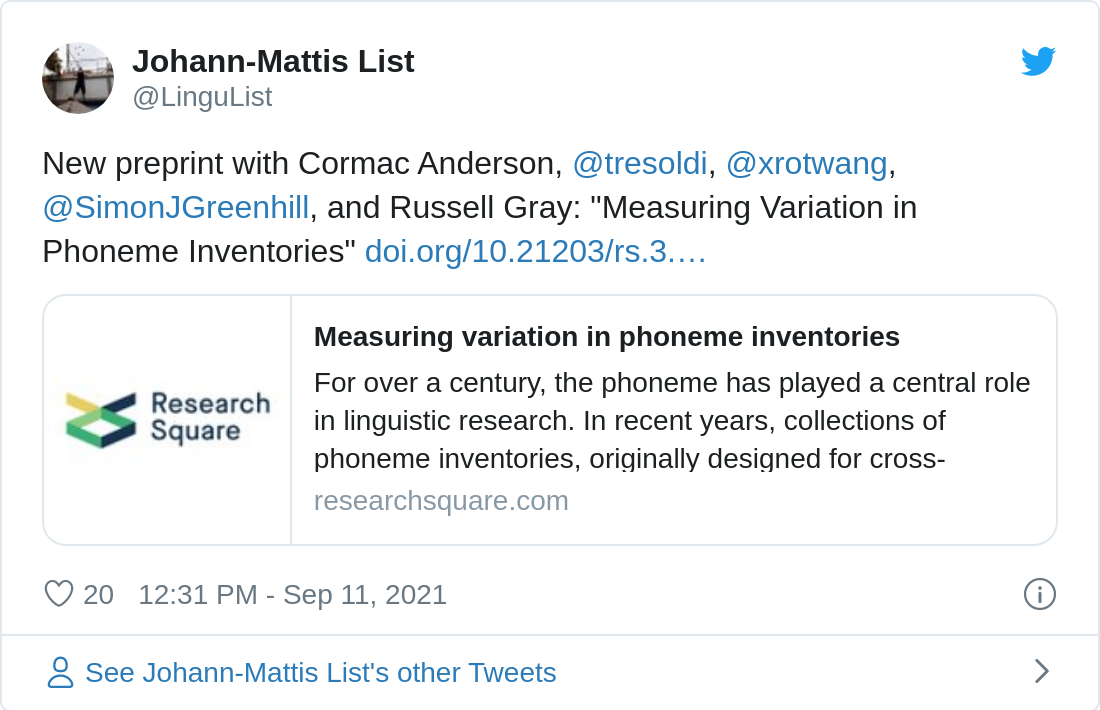
\includegraphics{2021.11.09_comparing_phonological_profiles_files/figure-beamer/list-1.png}
\end{frame}

\begin{frame}{How I decided to give this talk?}
\protect\hypertarget{how-i-decided-to-give-this-talk-1}{}
The main reason for this talk is that I performed calculation of
phonological distances (or caused people to do so) for Circassian
languages \citep{moroz21} and Andic branch of East Caucasian languages
\citep{moroz20, davidenko21, tsyzova21} in order to get a simple
less-connected to language phylogeny distance between different idioms.
\pause

But does this measure make any sense? How can we compare phonological
profiles of languages? \pause

Unlike lexicostatistical distance the phonological distance can be an
evidence for language contact, since languages can adopt some feature or
property of another (see \citep{andersson17}). This can be possible
explained by \textbf{Perceptual Magnet framework} \citep{blevins17}. In
most cases phonological change in unrelated languages is more salient to
linguists, however it is worth mentioning that there is a work about how
to catch contact-induced change in related languages \citep{bowern13}.
\end{frame}

\begin{frame}{Materials for the analysis}
\protect\hypertarget{materials-for-the-analysis}{}
Materials for the phonological distance calculation can be different:

\begin{itemize}
\tightlist
\item
  segment\footnote[frame]{Lets leave the phonology vs. phonetics debate aside.}
  inventory (and grammar, if you are lucky);
\item
  dictionaries;
\item
  parallel corpora;
\item
  unparalleled corpora.
\end{itemize}

\setcounter{footnote}{0}
\end{frame}

\hypertarget{criticism-by-simpson99}{%
\section{\texorpdfstring{Criticism by
\citep{simpson99}}{Criticism by {[}@simpson99{]}}}\label{criticism-by-simpson99}}

\begin{frame}{Criticism by \citep{simpson99}}
\protect\hypertarget{criticism-by-simpson99-1}{}
\citep{simpson99} attacks
UPSID\footnote[frame]{UPSID stands for UCLA Phonological Segment Inventory Database \citep{maddieson87} which consists of the phonemic systems of a
representative sample of 451 (this number changes from publication to publication) of the world's languages in machine-readable form. Now UPSID can be accessed via PHOIBLE database \citep{phoible19}.}-like
researches:

\begin{itemize}
\tightlist
\item
  phoneme masks allophones

  \begin{itemize}
  \tightlist
  \item
    Standard High German /ç/ stands for {[}ç{]}, {[}x{]} and {[}χ{]};
  \item
    ``The allophone no longer represents the phoneme, it \emph{replaces}
    it'';
  \end{itemize}
\item
  phonological relations between segments is lost

  \begin{itemize}
  \tightlist
  \item
    comparing just vowel inventories it is impossible to get information
    about e. g. vowel harmony;
  \end{itemize}
\item
  there is no non-arbitrary way of assign phonological features (e. g.
  SPE \citep{chomsky68}) to segments. \pause
\end{itemize}

My metaphor: omelet and pancakes share all ingredients, but they are
significantly different meals.

\setcounter{footnote}{0}
\end{frame}

\hypertarget{complexity-based-approaches}{%
\section{Complexity based
approaches}\label{complexity-based-approaches}}

\begin{frame}{\citep{pellegrino09} and \citep{sampson09}}
\protect\hypertarget{pellegrino09-and-sampson09}{}
\begin{center}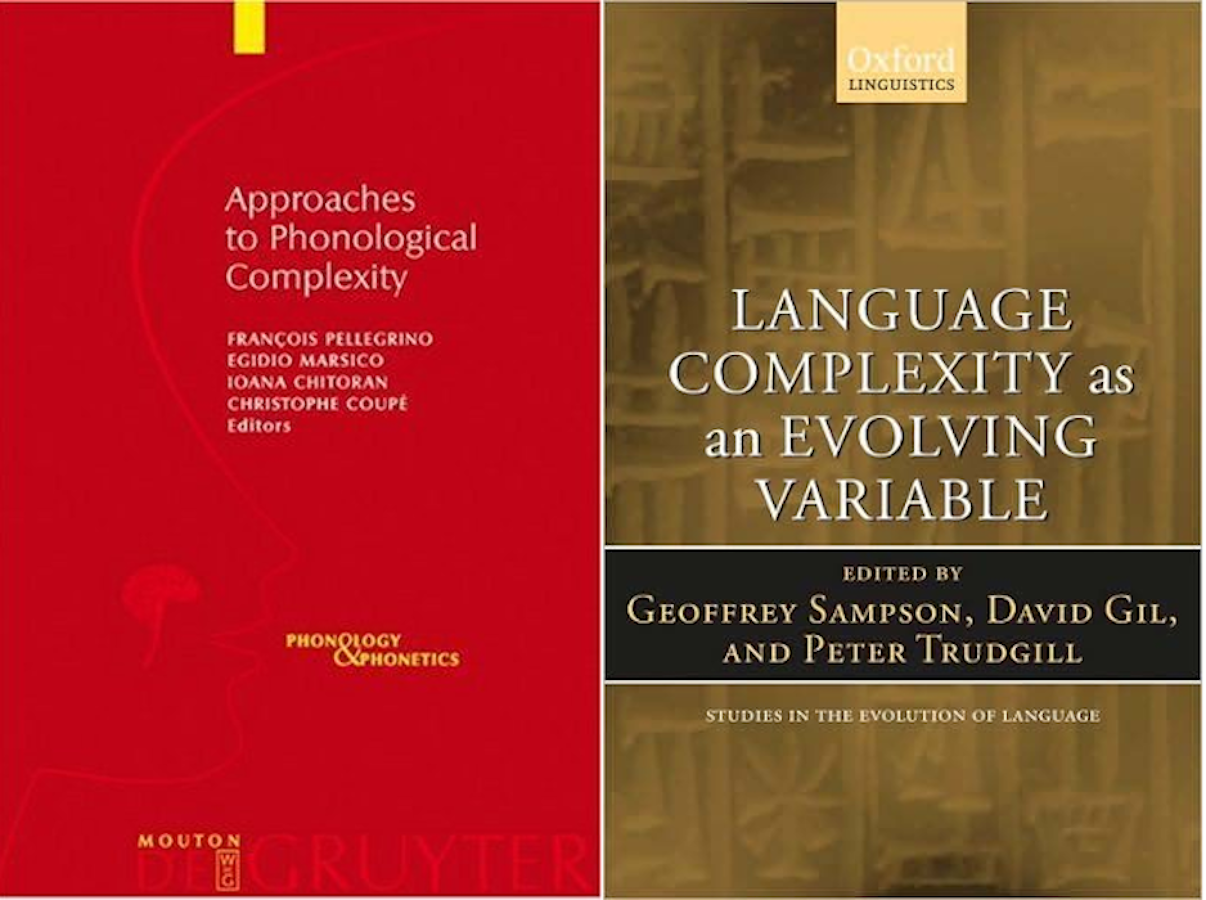
\includegraphics[width=16.75in]{images/complexity} \end{center}
\end{frame}

\begin{frame}{\citep{pellegrino09} and \citep{sampson09}}
\protect\hypertarget{pellegrino09-and-sampson09-1}{}
\begin{itemize}
\tightlist
\item
  \citep{pellegrino09}

  \begin{itemize}
  \tightlist
  \item
    \citep{ohala09}
  \item
    \citep{maddieson09}
  \item
    \citep{coupe09}
  \end{itemize}
\item
  \citep{sampson09}

  \begin{itemize}
  \tightlist
  \item
    \citep{nichols09}
  \item
    \citep{deutscher09}
  \end{itemize}
\end{itemize}
\end{frame}

\begin{frame}{\citep{nichols09}}
\protect\hypertarget{nichols09}{}
The main goal of this paper is to calculate overall complexity for a
typological sample of languages based on phonology, synthesis,
classification (gender, numeral classifiers), syntax, and lexicon. The
main goal is too prove:

\begin{itemize}
\tightlist
\item
  that all languages \textbf{are not} equal in complexity;
\item
  that different parts of grammar \textbf{do not} compensate for
  complexity in other parts of grammar. \pause
\end{itemize}

\begin{block}{Phonological features in the}
\protect\hypertarget{phonological-features-in-the}{}
\begin{itemize}
\tightlist
\item
  number of contrastive manners of articulation in stops;
\item
  number of vowel quality distinctions;
\item
  tone system (none/simple/complex, after \citep{maddieson13b});
\item
  syllable structure (after \citep{maddieson13a}).
\end{itemize}
\end{block}
\end{frame}

\begin{frame}{\citep[116]{nichols09}: results}
\protect\hypertarget{nichols09-116-results}{}
\begin{center}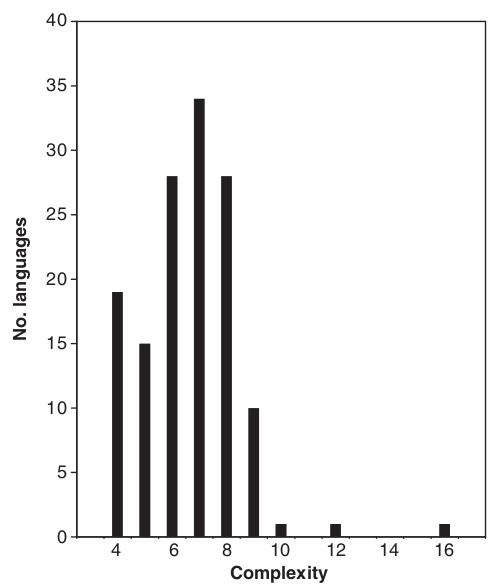
\includegraphics[width=2.52in]{images/nichols09} \end{center}

Phonological complexity (N = 137)
\end{frame}

\begin{frame}{\citep{ohala09}}
\protect\hypertarget{ohala09}{}
`Secondary distinctive features' are important for phonologization:

\begin{itemize}
\tightlist
\item
  nasals in French: saint {[}sɛ̃{]} \textless{} Latin sanctus `holy';
\item
  average F0 contour of vowels following English stops is falling after
  voiceless and rising after voiced.
\end{itemize}

They are not captured by the segmental inventories.

Allophones, like English /t/: {[}tʰ{]} vs {[}t{]} vs {[}ɾ{]} (cf
\citep{simpson99}).
\end{frame}

\begin{frame}{\citep{maddieson09}}
\protect\hypertarget{maddieson09}{}
\begin{itemize}
\tightlist
\item
  Merged measure for consonants, vowels, tones and syllable structure;
\end{itemize}

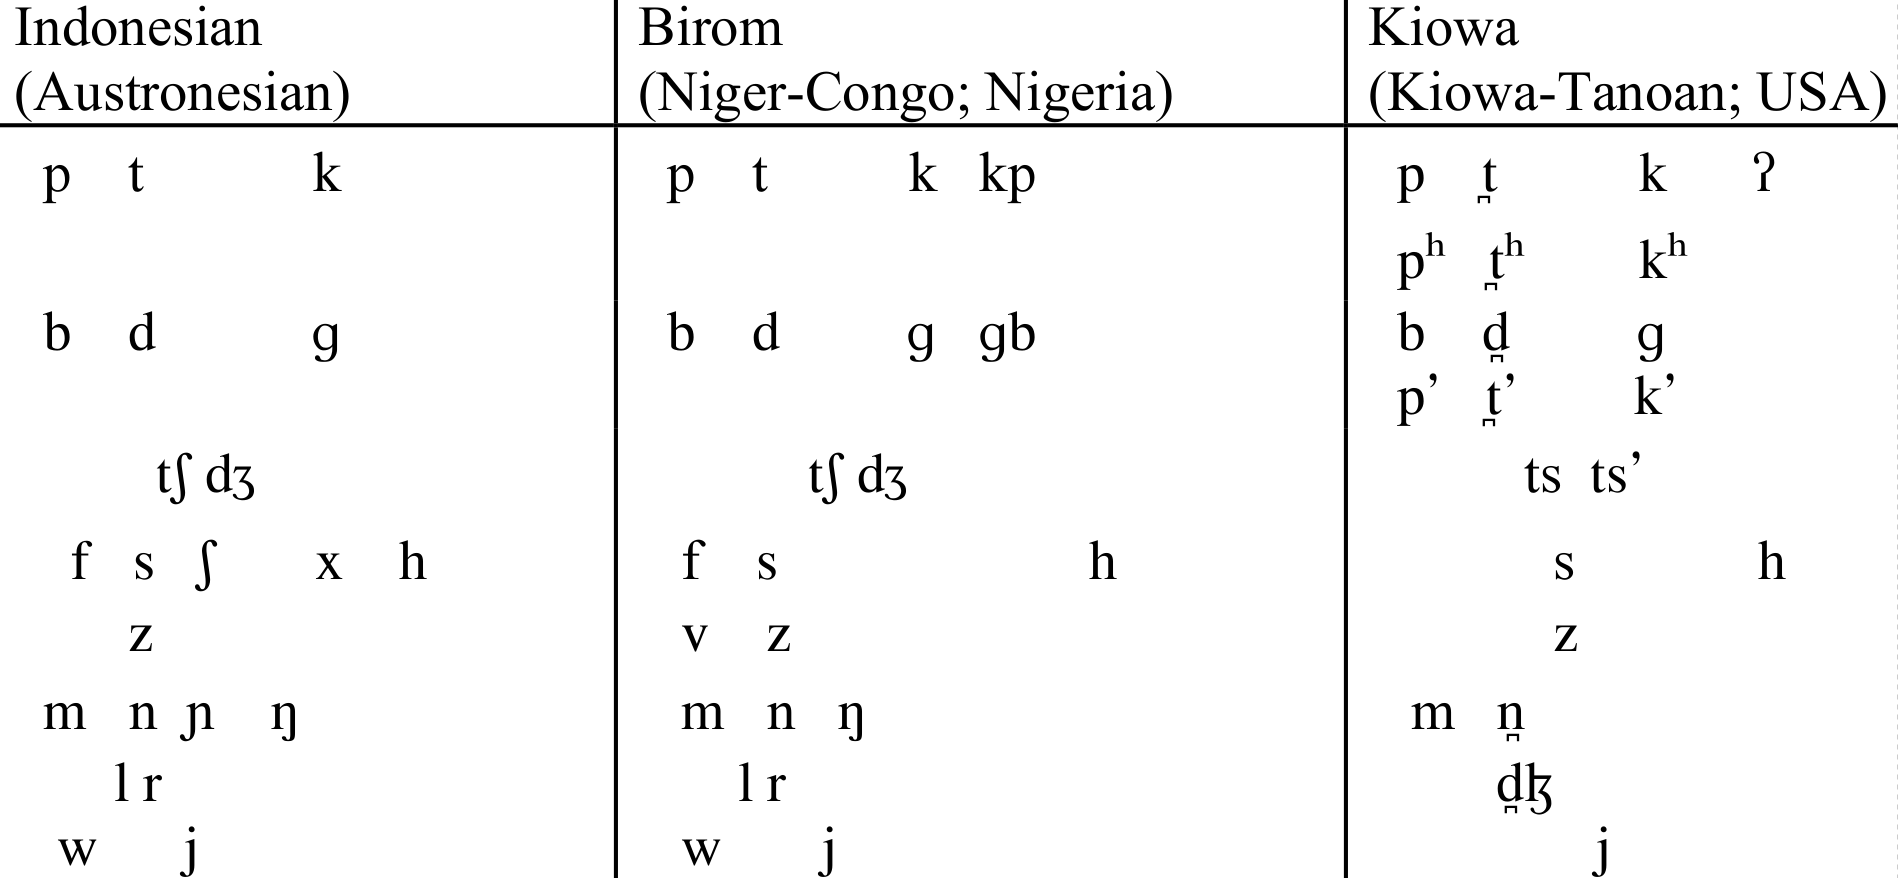
\includegraphics[width=4.52in]{images/maddieson09_ci}
\end{frame}

\begin{frame}{\citep{maddieson09}}
\protect\hypertarget{maddieson09-1}{}
\begin{itemize}
\tightlist
\item
  Merged measure for consonants, vowels, tones and syllable structure;
\end{itemize}

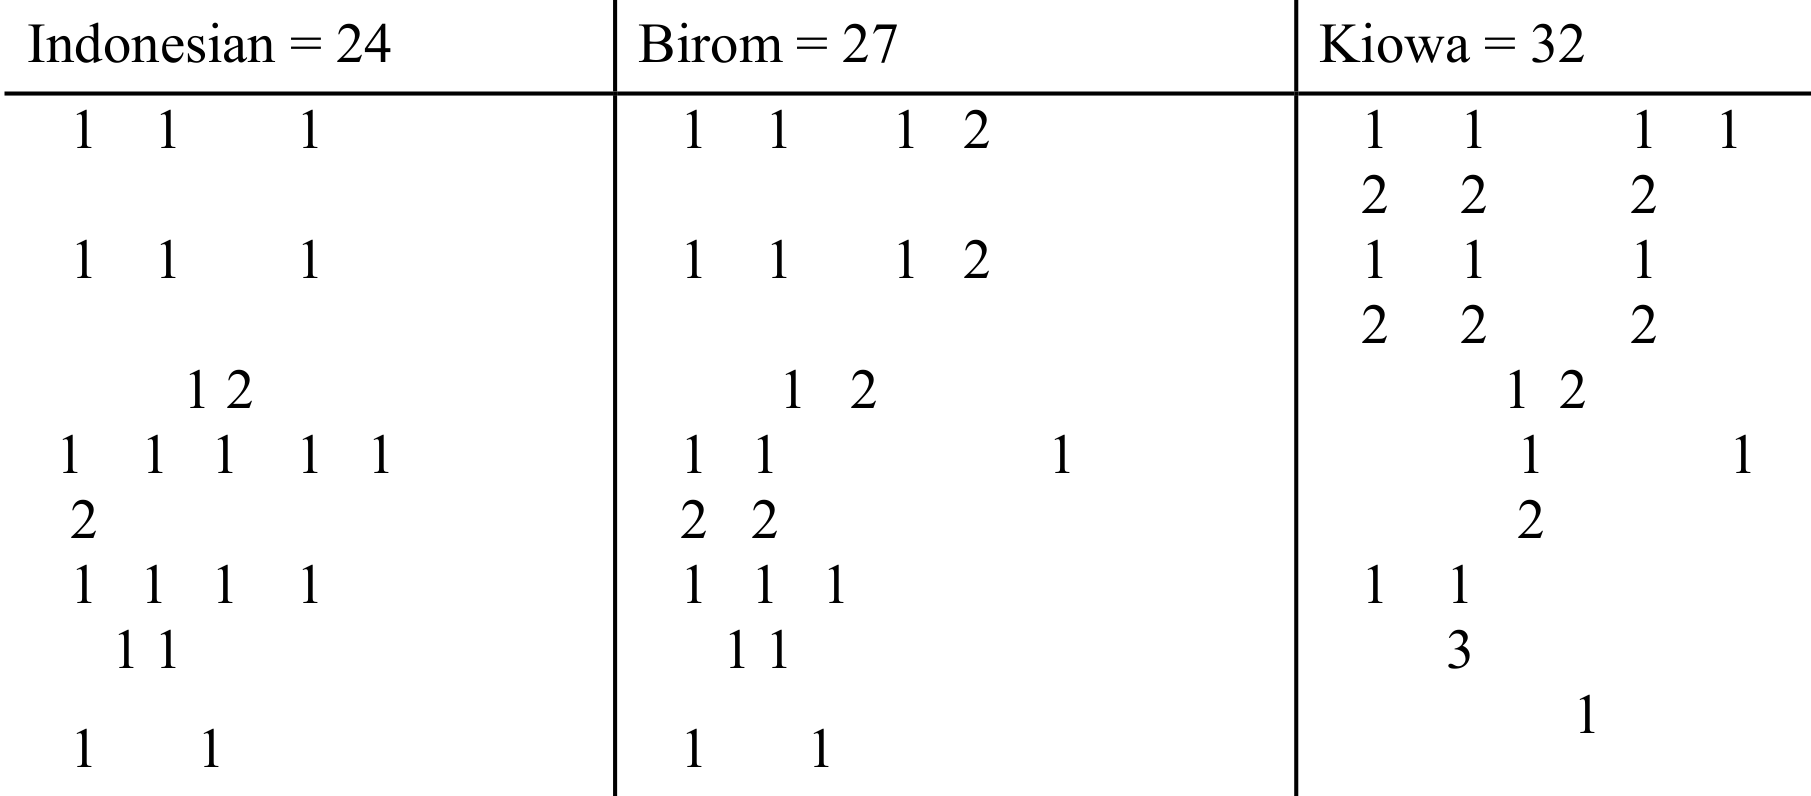
\includegraphics[width=4.31in]{images/maddieson09_cm}
\end{frame}

\begin{frame}{\citep{maddieson09}}
\protect\hypertarget{maddieson09-2}{}
\begin{itemize}
\tightlist
\item
  Merged measure for consonants, vowels, tones and syllable structure;
\item
  The number of possible distinct syllables allowed by the language (cf
  \citep{shosted06});
\item
  Frequency measures based on lexicon or texts (cf \citep{davidenko21}
  for Andic):
\end{itemize}

``To compare these data, it is useful to calculate some kind of index.
There are a number of ways this might be done. One possibility is to
calculate a summed frequency \(\times\) complexity score over the top
ten segments, in which each segment contributes decreasingly according
to its rank, and increasingly according to its complexity''.
\citep[97]{maddieson09}
\end{frame}

\begin{frame}{\citep{coupe09}}
\protect\hypertarget{coupe09}{}
\begin{itemize}
\tightlist
\item
  In this work authors use phonological features as a distances between
  segments and then use graphs with segments in the nodes and distances
  in the edges:
\end{itemize}

\begin{center}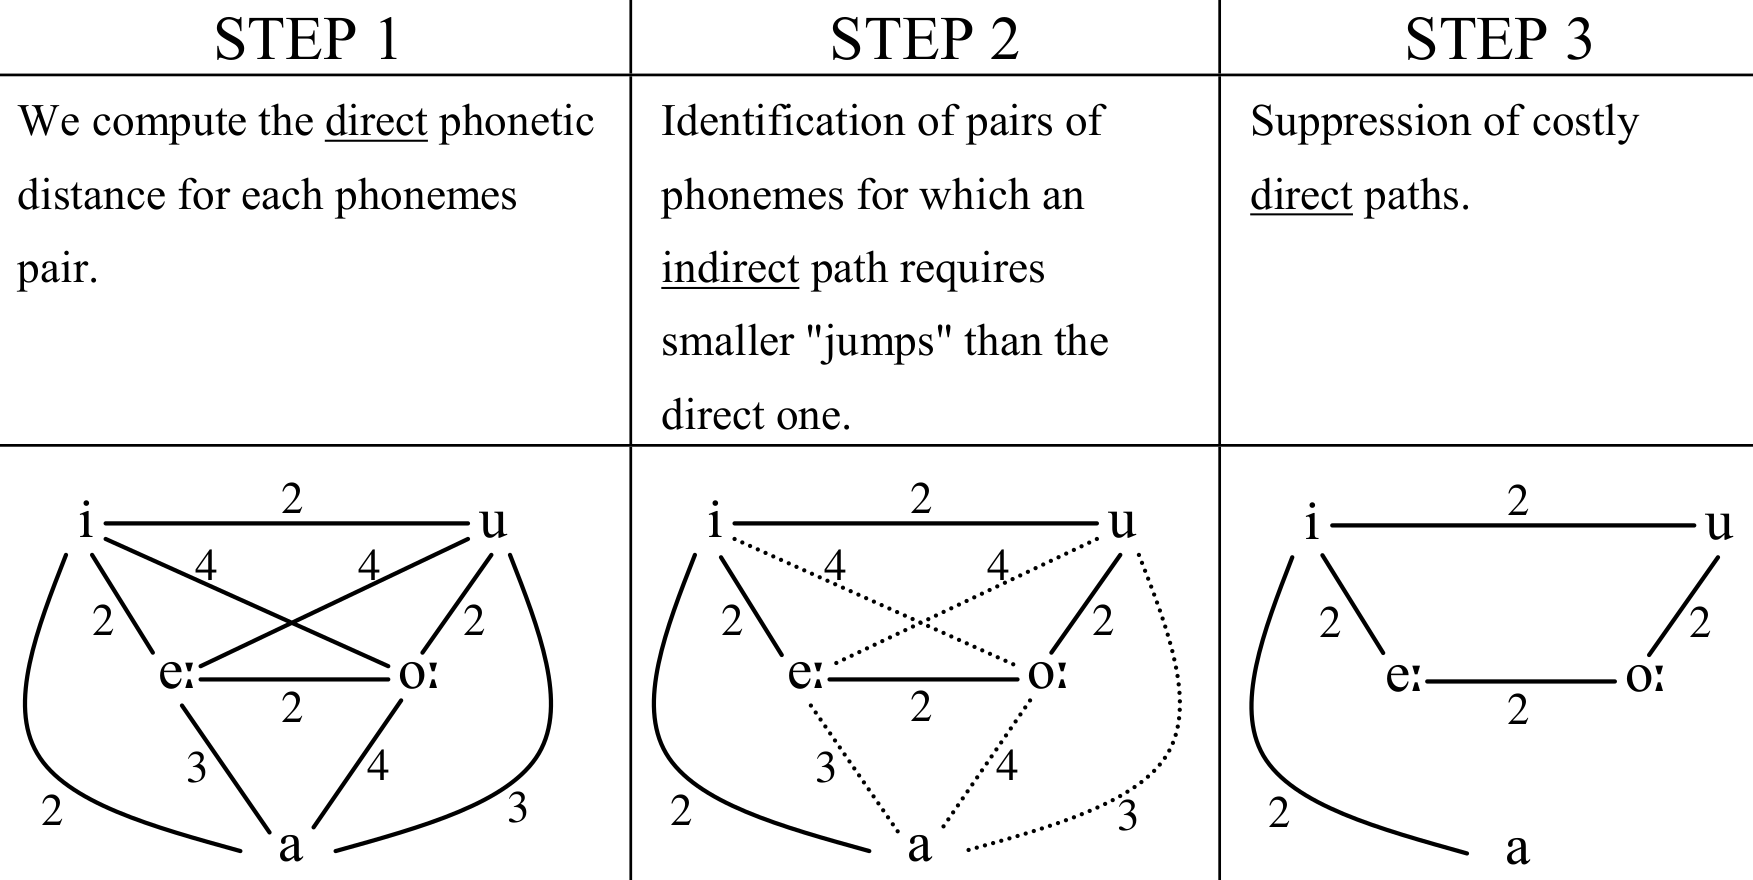
\includegraphics[width=4.61in]{images/coupe09} \end{center}
\end{frame}

\begin{frame}{\citep{coupe09}}
\protect\hypertarget{coupe09-1}{}
\begin{itemize}
\tightlist
\item
  In this work authors use phonological features as a distances between
  segments and then use graphs with segments in the nodes and distances
  in the edges.
\item
  Afterwords authors use \emph{off-diagonal complexity} proposed by
  \citep{claussen07}\footnote[frame]{Authors motivated their choice, because this measure
  \begin{itemize}
  \item does not explicitly take into account graph size;
  \item is sensitive to the presence of hierarchical sub-structures in the network;
  \item is minimal for regular graphs and maximal for free-scale graphs.
  \end{itemize}
  Unfortunately, off-diagonal complexity can not be calculated for valued graphs, so authors were ought to drop phonologcial distance values from their graphs.
  } that make it possible to disassociate from linguistics and phonology
  and rely purely on graph structure.
\end{itemize}

\setcounter{footnote}{0}
\end{frame}

\begin{frame}{\citep{deutscher09}}
\protect\hypertarget{deutscher09}{}
\begin{itemize}
\tightlist
\item
  `All Languages are Equally Complex' --- is a legend (actually, a lot
  of papers from \citep{sampson09} state the same).
\item
  Complexity is a polysemous notion: some scholars focus on multipartite
  nature of language, others on complicated relations within the system.
\item
  Overall complexity is better to present as a vector of values rather
  then one value.
\end{itemize}
\end{frame}

\begin{frame}{Conclusions}
\protect\hypertarget{conclusions}{}
Despite of the critics that language phonological system is a complex
system that can not be reduced to the set of its elements
\citep{simpson99, ohala09, coupe09, deutscher09} I think that any
phonological complexity measure can be used in order to compare
different languages. The sophistication and granularity of this measure
will influence the possible effect size gathered by this measure.
\end{frame}

\hypertarget{distance-based-approaches}{%
\section{Distance based approaches}\label{distance-based-approaches}}

\begin{frame}{Distance based approaches}
\protect\hypertarget{distance-based-approaches-1}{}
\begin{itemize}
\tightlist
\item
  \citep{hoppenbrouwers01} (after \citep{heeringa04})
\item
  \citep{nerbonne01}
\item
  \citep{heeringa04}
\item
  \citep{eden18}
\item
  \citep{anderson21}
\end{itemize}
\end{frame}

\begin{frame}{\citep{anderson21}}
\protect\hypertarget{anderson21}{}
In this paper authors apply \textbf{Jaccard similarity} between two
phoneme inventories, that is ratio of similar segments in two languages
out of all possible segments in two languages. \pause

The reason, why authors do that is because their goal is to compare
different inventories of the \textbf{same} languages across four
databases of phonological inventories (UPSID \citep{maddieson87}, LAPSyD
\citep{maddieson13}, Core PHOIBLE \citep{phoible19}, JIPA
\citep{baird21}). The results are unfavorable: researchers found a high
degree of variation across datasets.
\end{frame}

\begin{frame}{\citep{hoppenbrouwers01} after \citep{heeringa04}}
\protect\hypertarget{hoppenbrouwers01-after-heeringa04}{}
\begin{itemize}
\tightlist
\item
  Extract unit (it can be segments, syllables or phonological features)
  frequencies from corpora or dictionary.
\item
  The distance between two languages is the sum of the differences
  between the corresponding unit frequencies.
\end{itemize}
\end{frame}

\begin{frame}{\citep{nerbonne01} after \citep{heeringa04}}
\protect\hypertarget{nerbonne01-after-heeringa04}{}
Authors applied the same stratagy as \citep{hoppenbrouwers01}, but used
words as a corpora. So the idiom distance is calculated as an average
word distance.
\end{frame}

\begin{frame}{\citep{heeringa04}}
\protect\hypertarget{heeringa04}{}
Since \citep{hoppenbrouwers01} and \citep{nerbonne01} methods does not
account for unit order Heeringa decided to use Levenstein distance
\citep{levenstein65}. The Levenstein distance is the minimum number of
unit edits (insertions, deletions or substitutions) that should be
applied to the unit string in order to get another:

\begin{itemize}
\tightlist
\item
  the distance between \emph{sing} and \emph{king} is 1
\item
  the distance between \emph{sing} and \emph{sign} is 1
\item
  the distance between \emph{sing} and \emph{sight} is 3
\end{itemize}

Shortcoming:

\begin{itemize}
\tightlist
\item
  diphthong vs.~vowel + consonant combination (/au/ or /aw/?);
\item
  suprasegmental features;
\item
  sequence length: the longer the sequences, the greater the chance of
  differences between them.
\end{itemize}
\end{frame}

\begin{frame}{\citep{heeringa04}}
\protect\hypertarget{heeringa04-1}{}
To address the sequence length problem \citep{heeringa04} uses
normalization by the length of the alignment:

\begin{center}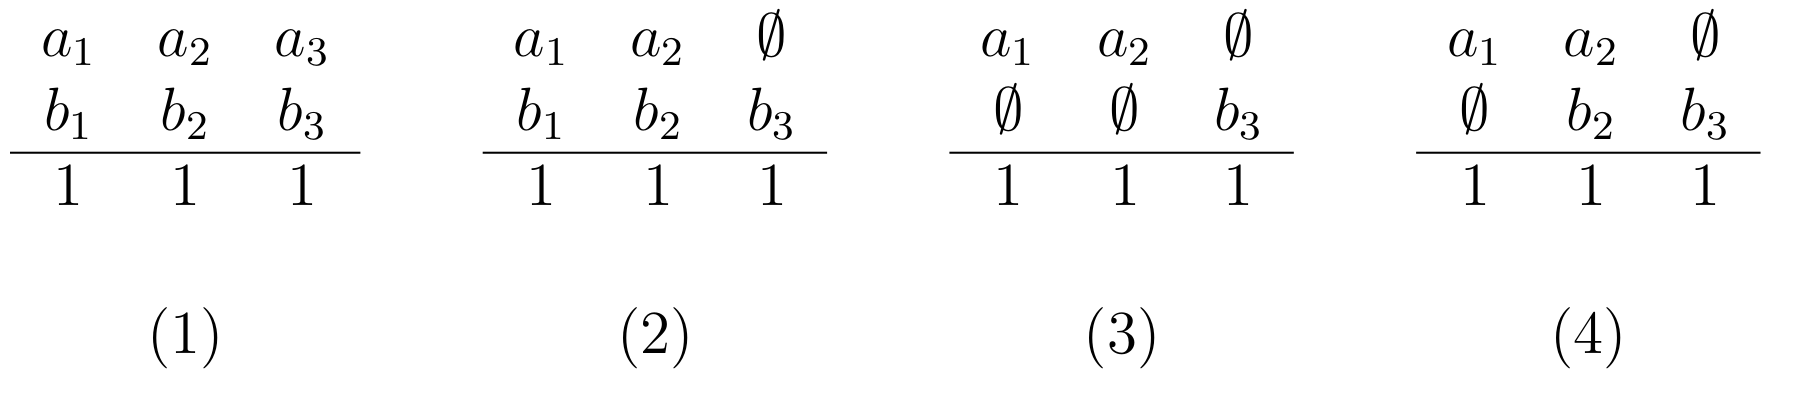
\includegraphics[width=4.52in]{images/heeringa04_norm} \end{center}

All four examples are normalized by the value 3.
\end{frame}

\begin{frame}{\citep{heeringa04}: interlanguage stimuli mismatch}
\protect\hypertarget{heeringa04-interlanguage-stimuli-mismatch}{}
\begin{itemize}
\tightlist
\item
  It is possible that for one of the pair of idioms one lack stimuli,
  then the effect of this stimuli is discounted.
\item
  In case of multiple transcription they are matched according the
  minimum distance:

  \begin{itemize}
  \tightlist
  \item
    L1: {[}hys{]}; L2: {[}hys{]} and {[}hus{]}
  \item
    L1: {[}hys{]} and {[}hus{]}; L2: {[}hys{]} and {[}hus{]}
  \end{itemize}
\end{itemize}
\end{frame}

\begin{frame}{\citep{eden18}}
\protect\hypertarget{eden18}{}
\end{frame}

\begin{frame}{Conclusions}
\protect\hypertarget{conclusions-1}{}
\end{frame}

\begin{frame}{}
\protect\hypertarget{section}{}
\LARGE Thank you for your attention!
\end{frame}

\renewcommand\refname{References}
\begin{frame}[allowframebreaks]{References}
  \bibliographytrue
  \bibliography{bibliography.bib}
\end{frame}

\end{document}
